\documentclass[a4paper,11pt]{book}

%%%%%%%%%%%%%%%%%%%%%%%%%%%%%%%%%
% Paquetes
%%%%%%%%%%%%%%%%%%%%%%%%%%%%%%%%%
\usepackage[utf8]{inputenc}
\usepackage[spanish]{babel}
\usepackage{csquotes}
\usepackage[inline]{enumitem}
\usepackage{graphicx}
\usepackage[official]{eurosym}
\usepackage{listings}

\decimalpoint
\usepackage{dcolumn}
\newcolumntype{.}{D{.}{\esperiod}{-1}}
\makeatletter
\addto\shorthandsspanish{\let\esperiod\es@period@code}
\makeatother

\RequirePackage{verbatim}
\usepackage{fancyhdr}
\usepackage{afterpage}
\usepackage{longtable}
\usepackage[pdfborder={0 0 0}]{hyperref} %referencia
\usepackage{url}
\usepackage{colortbl}
\usepackage[stable]{footmisc}
\usepackage{pdfpages}

% ********************************************************************
% Re-usable information
% ********************************************************************

\newcommand{\myTitle}{Desarrollo de un instrumento musical digital\xspace}
\newcommand{\myDegree}{Grado en ...\xspace}
\newcommand{\myName}{Jesús Jiménez Sánchez (alumno)\xspace}
\newcommand{\myProf}{Alberto Guillén Perales (tutor1)\xspace}
%\newcommand{\mySupervisor}{Put name here\xspace}
\newcommand{\myFaculty}{Escuela Técnica Superior de Ingenierías Informática y de Telecomunicación\xspace}
\newcommand{\myFacultyShort}{E.T.S. de Ingenierías Informática y de Telecomunicación\xspace}
\newcommand{\myDepartment}{Departamento de ...\xspace}
\newcommand{\myUni}{\protect{Universidad de Granada}\xspace}
\newcommand{\myLocation}{Granada\xspace}
\newcommand{\myTime}{\today\xspace}
\newcommand{\myVersion}{Version 0.1\xspace}


%%%%%%%%%%%%%%%%%%%%%%%%%%%
% Preparar pdf
%%%%%%%%%%%%%%%%%%%%%%%%%%%

\hypersetup{
    pdfauthor = {\myName (jesusjimsacorreo.ugr.es)},
    pdftitle = {\myTitle},
    pdfsubject = {},
    pdfkeywords = {palabraclave1, palabraclave2, palabraclave3, ...},
    pdfcreator = {LaTeX con el paquete ....},
    pdfproducer = {pdflatex}
}



% Comandos útiles
\pagestyle{fancy}
\fancyhf{}
\fancyhead[LO]{\leftmark}
\fancyhead[RE]{\rightmark}
\fancyhead[RO,LE]{\textbf{\thepage}}
\renewcommand{\chaptermark}[1]{\markboth{\textbf{#1}}{}}
\renewcommand{\sectionmark}[1]{\markright{\textbf{\thesection. #1}}}

\setlength{\headheight}{1.5\headheight}

\newcommand{\HRule}{\rule{\linewidth}{0.5mm}}
% Definimos los tipos teorema, ejemplo y definición podremos usar estos tipos
% simplemente poniendo \begin{teorema} \end{teorema} ...
\newtheorem{teorema}{Teorema}[chapter]
\newtheorem{ejemplo}{Ejemplo}[chapter]
\newtheorem{definicion}{Definición}[chapter]

\definecolor{gray97}{gray}{.97}
\definecolor{gray75}{gray}{.75}
\definecolor{gray45}{gray}{.45}
\definecolor{gray30}{gray}{.94}

\lstset{
    frame=Ltb,
    framerule=0.5pt,
    aboveskip=0.5cm,
    framextopmargin=3pt,
    framexbottommargin=3pt,
    framexleftmargin=0.1cm,
    framesep=0pt,
    rulesep=.4pt,
    backgroundcolor=\color{gray97},
    rulesepcolor=\color{black},
    %
    stringstyle=\ttfamily,
    showstringspaces = false,
    basicstyle=\scriptsize\ttfamily,
    commentstyle=\color{gray45},
    keywordstyle=\bfseries,
    %
    numbers=left,
    numbersep=6pt,
    numberstyle=\tiny,
    numberfirstline = false,
    breaklines=true,
}

% minimizar fragmentado de listados
\lstnewenvironment{listing}[1][]
   {\lstset{#1}\pagebreak[0]}{\pagebreak[0]}

\lstdefinestyle{CodigoC}
   {
	basicstyle=\scriptsize,
	frame=single,
	language=C,
	numbers=left
   }

\lstdefinestyle{CodigoC++}
   {
	basicstyle=\small,
	frame=single,
	backgroundcolor=\color{gray30},
	language=C++,
	numbers=left
   }

\lstdefinestyle{Consola}
   {
    basicstyle=\scriptsize\bf\ttfamily,
    backgroundcolor=\color{gray30},
    frame=single,
    numbers=none
   }


\newcommand{\bigrule}{\titlerule[0.5mm]}

%Para conseguir que en las páginas en blanco no ponga cabecerass
\makeatletter
\def\clearpage{%
    \ifvmode
        \ifnum \@dbltopnum =\m@ne
        \ifdim \pagetotal <\topskip
            \hbox{}
        \fi
        \fi
    \fi
    \newpage
    \thispagestyle{empty}
    \write\m@ne{}
    \vbox{}
    \penalty -\@Mi
}
\makeatother

%%%%%%%%%%%%%%%%%%%%%%%%%%%%%%%%%%
% Imagenes
%%%%%%%%%%%%%%%%%%%%%%%%%%%%%%%%%%
\graphicspath{ {./imagenes/} }


\title{ \myTitle }
\author{ \myName }

\begin{document}

\begin{titlepage}
 
 
\newlength{\centeroffset}
\setlength{\centeroffset}{-0.5\oddsidemargin}
\addtolength{\centeroffset}{0.5\evensidemargin}
\thispagestyle{empty}

\noindent\hspace*{\centeroffset}\begin{minipage}{\textwidth}

\centering

\includegraphics[width=0.9\textwidth]{logo_ugr.jpg}\\[1.4cm]

\textsc{ \Large TRABAJO FIN DE GRADO\\[0.2cm]}
\textsc{ INGENIERÍA EN INGENIERÍA INFORMÁTICA}\\[1cm]
% Upper part of the page
% 
% Title
{\Huge\bfseries Desarrollo de un instrumento musical digital\\
}
\noindent\rule[-1ex]{\textwidth}{3pt}\\[3.5ex]
{\large\bfseries Subtitulo del Proyecto}
\end{minipage}

\vspace{2.5cm}
\noindent\hspace*{\centeroffset}\begin{minipage}{\textwidth}
\centering

\textbf{Autor}\\ { Jesús Jiménez Sánchez (alumno) }\\[2.5ex]
\textbf{Directores}\\
{ Alberto Guillén Perales \\[2cm] }

\includegraphics[width=0.3\textwidth]{etsiit_logo.png}\\[0.1cm]
\textsc{Escuela Técnica Superior de Ingenierías Informática y de Telecomunicación}\\
\textsc{---}\\
Granada, mes de 201
\end{minipage}

\end{titlepage}



%%%%%%%%%%%%%%%%%%%%%%%%%%%%%%%%%%%%%%%%%%%%%%%%%%%%%%%%%%%%%%%%%%%%%%%%%%%%%%%%%
% Prefacio
%%%%%%%%%%%%%%%%%%%%%%%%%%%%%%%%%%%%%%%%%%%%%%%%%%%%%%%%%%%%%%%%%%%%%%%%%%%%%%%%%

\chapter*{}   %%%%%%%%%%%%%%%%%%%%%%

\cleardoublepage
\thispagestyle{empty}

\begin{center}
    {\large\bfseries Desarrollo de un instrumento musical digital}\\
\end{center}

\begin{center}
    Jesús Jiménez Sánchez\\
\end{center}

%\vspace{0.7cm}
\noindent{\textbf{Palabras clave}: batería, sonido, Raspberry, Arduino, ......}\\

\vspace{0.7cm}
\noindent{\textbf{Resumen}}\\

Poner aquí el resumen.

\cleardoublepage

\thispagestyle{empty}

\begin{center}
       {\large\bfseries Development of a digital musical instrument}\\
\end{center}

\begin{center}
    Jesús Jiménez Sánchez\\
\end{center}

\noindent{\textbf{Keywords}: batería, sonido, Raspberry, Arduino, ....}\\

\vspace{0.7cm}
\noindent{\textbf{Abstract}}\\

Write here the abstract in English.

\chapter*{}   %%%%%%%%%%%%%%%%%%%%%%

\thispagestyle{empty}

\noindent\rule[-1ex]{\textwidth}{2pt}\\[4.5ex]

Yo, \textbf{Jesús Jiménez Sánchez}, alumno de la titulación \textbf{Grado en Ingeniería Informática} de la
\textbf{Escuela Técnica Superior de Ingenierías Informática y de Telecomunicación de la Universidad de Granada}, con DNI
11111111A, autorizo la ubicación de la siguiente copia de mi Trabajo Fin de Grado en la biblioteca del centro para que
pueda ser consultada por las personas que lo deseen.

\vspace{6cm}

\noindent Fdo: Jesús Jiménez Sánchez

\vspace{2cm}

\begin{flushright}
    Granada a X de mes de 2020.
\end{flushright}

\chapter*{}   %%%%%%%%%%%%%%%%%%%%%%
\thispagestyle{empty}

\noindent\rule[-1ex]{\textwidth}{2pt}\\[4.5ex]

D. \textbf{Alberto Guillén Perales}, Profesor del Área de XXXX del Departamento YYYY de la Universidad de
Granada.

\vspace{0.5cm}

\textbf{Informan:}

\vspace{0.5cm}

Que el presente trabajo, titulado \textit{\textbf{Desarrollo de un instrumento musical digital}},
ha sido realizado bajo su supervisión por \textbf{Jesús Jiménez Sánchez}, y autorizamos la defensa de
dicho trabajo ante el tribunal
que corresponda.

\vspace{0.5cm}

Y para que conste, expiden y firman el presente informe en Granada a X de mes de 201 .

\vspace{1cm}

\textbf{Los directores:}

\vspace{5cm}

\noindent \textbf{Alberto Guillén Perales}

\chapter*{Agradecimientos}  %%%%%%%%%%%%%%%%%%%%%%
\thispagestyle{empty}

    \vspace{1cm}


Poner aquí agradecimientos...


\newpage
\tableofcontents
\newpage

%%%%%%%%%%%%%%%%%%%%%%%%%%%%%%%%%%%%%%%%%%%%%%%%%%%%%%%%%%%%%%%%%%%%%%%%%%%%%%%%%
% Objetivos
%%%%%%%%%%%%%%%%%%%%%%%%%%%%%%%%%%%%%%%%%%%%%%%%%%%%%%%%%%%%%%%%%%%%%%%%%%%%%%%%%

\chapter{Objetivos} % (fold)
\label{cha:Objetivos}

    Objetivo General:

    Objetivos específicos:
    \begin{itemize}
        \item OB-E1: Planificación
        \item OB-E2:
    \end{itemize}

% chapter Objetivos (end)


%%%%%%%%%%%%%%%%%%%%%%%%%%%%%%%%%%%%%%%%%%%%%%%%%%%%%%%%%%%%%%%%%%%%%%%%%%%%%%%%%
% Introducción
%%%%%%%%%%%%%%%%%%%%%%%%%%%%%%%%%%%%%%%%%%%%%%%%%%%%%%%%%%%%%%%%%%%%%%%%%%%%%%%%%

\chapter{Introducción} % (fold)
\label{cha:Introduccion}

    \section{Historia de los instrumentos digitales} % (fold)
    \label{sec:HistoriaDeLosInstrumentosDigitales}

        Los primeros intentos de guardar y reproducir el sonido fueron analógicos. Estos métodos captan las ondas y las
        almacenan en diferentes medios para su posterior reproducción, como en un disco de vinilo o un casete.

        Con la aparición de la informática y los ordenadores se empiezan a almacenar estos sonidos en un formato
        digital, capaz de ser interpretado por ordenadores. En este caso, los sonidos se guardan en forma de bytes en
        diferentes formatos de archivo, como MP3, AAC, OGG...

        Los primeros intentos de instrumento musical no analógico se pueden encontrar en los sintetizadores. Estos
        intrumentos utilizan la electricidad para producir las ondas del sonidos pasándola por una serie de módulos.
        Hasta la década de 1980, cada fabricante utilizaba su propio estándar para la sincronización de los sonidos de
        los sintetizadores. En 1981, la empresa Oberheim Electronics comenzó a contactar con otros fabricantes para
        desarrollar un estándar, de ese modo apareció MIDI. Este estándar describe el protocolo de comunicación, la
        interfaz digital y las conexiones electrónicas que deben llevar los diferentes tipos de dispositivos
        electrónicos para reproducir, editar y grabar música \cite{midi_wikipedia}.

        En cuanto a instrumentos musicales electrónicos podemos encontrar desde un teclado o una guitarra a una batería.

        En el área de instrumentos digitales nos encontramos con los instrumentos VST (Virtual Studio Technology). Estos
        instrumentos toman muestras de sonidos de diferentes instrumentos y, mediante un teclado y un ordenador,
        programar estos sonidos y componer y grabar cualquier tipo de canción \cite{historia_instrumentos_digitales}.

        \newpage

        \begin{figure}[ht]
            \centering
            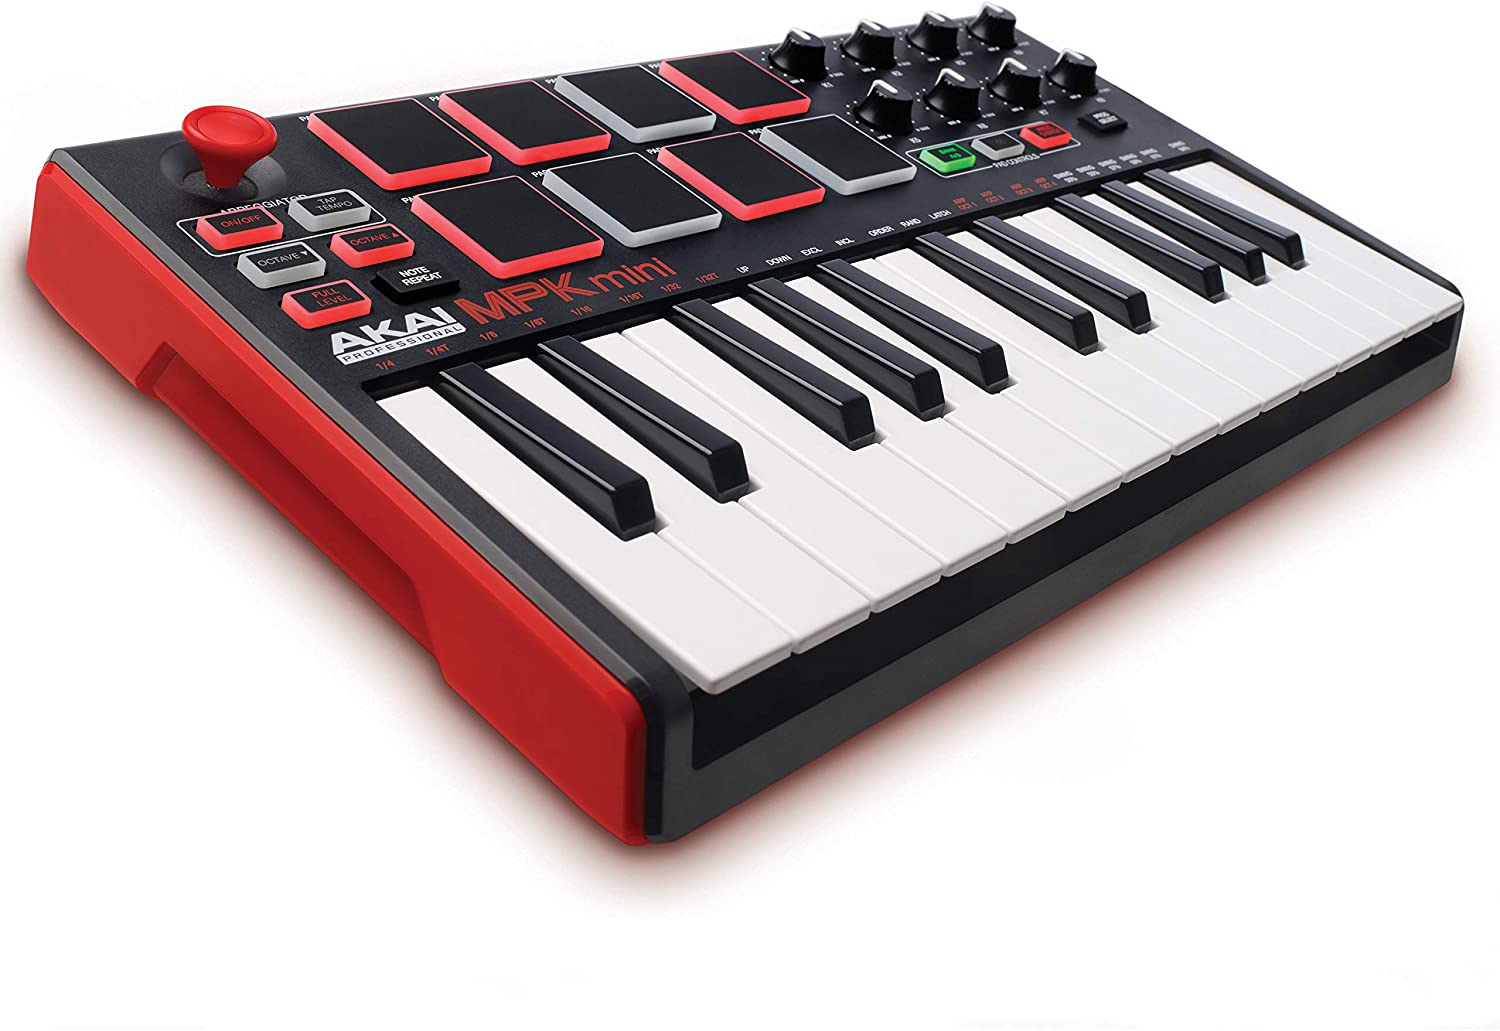
\includegraphics[width=\textwidth/2]{ejemplo_sampler}
            \caption{Ejemplo de sampler digital de la marca AKAI Pro \cite{akai_pro_imagen}\label{fig:EjemploSampler}}
        \end{figure}

    % section Historia de los instrumentos digitales (end)

    \section{Partes de una batería} % (fold)
    \label{sec:PartesDeUnaBateria}

        Las partes de una batería son las siguientes:

        \begin{itemize}
            \item \textbf{Caja}: Su función principal suele ser la de marcar los compases.
            \item \textbf{Toms}: Son los tambores más numerosos en una batería.
            \item \textbf{Bombo}: Se toca con un pedal y produce el sonido más grave de la batería. Se utiliza para
            llevar la base del ritmo.
            \item \textbf{Platillo crash}: Se utiliza para dar énfasis y suele ir acompañado del bombo.
            \item \textbf{Platillo hi-hat}: Consta de dos platillos que se pueden abrir o cerrar con un pedal y se
            utiliza para llevar el ritmo de la canción.
            \item \textbf{Platillo ride}: Puede usarse para llevar el ritmo en lugar de con el hi-hat.
        \end{itemize}

        \newpage

        \begin{figure}[ht]
            \centering
            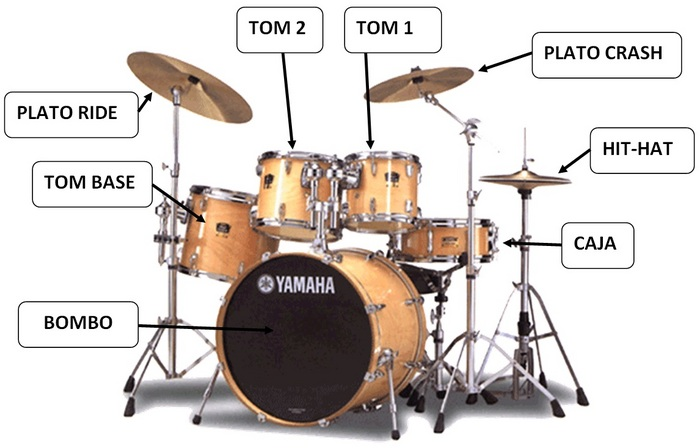
\includegraphics[width=10cm]{partes_bateria}
            \caption{Partes de una batería \cite{partes_bateria_fuente}\label{fig:PartesBateria}}
        \end{figure}

    % section Partes de una batería (end)

    \section{Etapas} % (fold)
    \label{sec:Etapas}

        \begin{itemize}
            \item \textbf{1ª etapa:} Estudio del problema.

            \item \textbf{2ª etapa:} Búsqueda de bibliotecas de reproducción de sonido.

            \item \textbf{3ª etapa:} Implementación del software.

            \item \textbf{4 a etapa:} Construcción de la batería.

            \item \textbf{5ª etapa:} Documentación.
        \end{itemize}

    % section Etapas (end)

    \section{Planificación} % (fold)
    \label{sec:Planificacion}

        \subsection{A priori optimista} % (fold)
        \label{sub:APrioriOptimista}

            \begin{figure}[ht]
                \centering
                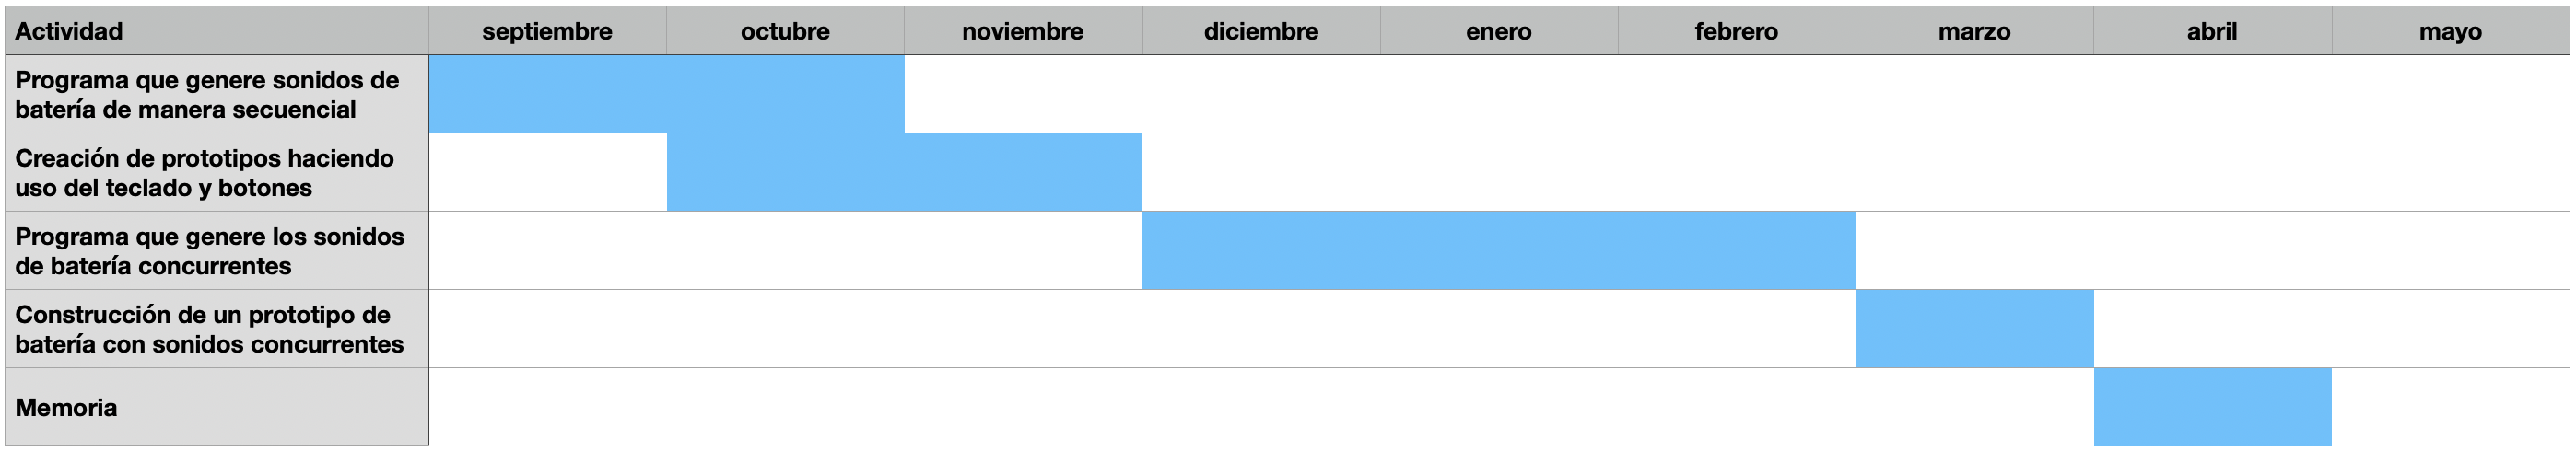
\includegraphics[width=\textwidth]{planificacion_gantt}
                \caption{Diagrama de Gantt de la planificación por etapas\label{fig:PlanificacionGantt}}
            \end{figure}

        % subsection A priori optimista (end)

        % \subsection{A posteriori (en caso de haber diferencias)} % (fold)
        % \label{sub:APosterioriEnCasoDeHaberDiferencias)}

        % subsection A posteriori (en caso de haber diferencias) (end)

    % section Planificación (end)

% chapter Introducción (end)

\newpage

%%%%%%%%%%%%%%%%%%%%%%%%%%%%%%%%%%%%%%%%%%%%%%%%%%%%%%%%%%%%%%%%%%%%%%%%%%%%%%%%%
% Aspectos legales
%%%%%%%%%%%%%%%%%%%%%%%%%%%%%%%%%%%%%%%%%%%%%%%%%%%%%%%%%%%%%%%%%%%%%%%%%%%%%%%%%

\chapter{Aspectos legales} % (fold)
\label{cha:AspectosLegales}

    \section{Derechos de autor} % (fold)
    \label{sec:DerechosDeAutor}
        \subsection{¿Qué son los derechos de autor?} % (fold)
        \label{sub:QueSonLosDerechosDeAutor}

            Los derechos de autor son una serie de leyes que protegen la autoría de las obras. Estas pueden ser libros,
            películas, obras de teatro, programas informáticos...\newline

            Se cubren dos tipos de derechos: los derechos patrimoniales, que aseguran que el autor obtenga compensación
            financiera, y los derechos morales, que cubren todo lo que no esté relacionado con los derechos
            patrimoniales, por ejemplo, la prohibición de que se modifique la obra.\cite{derechos_ompi}

        % section ¿Qué son los derechos de autor? (end)

        \subsection{Historia de los derechos de autor} % (fold)
        \label{sub:HistoriaDeLosDerechosDeAutor}

            La historia de los derechos de autor comienza en 1710, cuando se publica el Estatuto de la Reina
            Anna\cite{estatuto_anna} que fue el primer reglamento sobre los derechos de autor. En el momento de la
            publicación de éste estatuto solo se contemplaban los derechos sobre los libros, pero en posteriores leyes
            se contemplan otros usos, como cine, radio, fotografías o programas de ordenador.\newline

            En la actualidad, los derechos de autor se protegen tanto con acuerdos y leyes internacionales, como leyes
            nacionales.\newline

            Desde 1974 en Estados Unidos con la CONTU\cite{contu} (Commission on New Technological Uses of Copyrighted
            Works) y de 1991 en la Unión Europea con la Computer Programs Directive\cite{com_pro_dir}, se protegen los
            derechos de autor de los programas informáticos.

        % subsection Historia de los derechos de autor (end)
    
    % section Derechos de autor (end)

    \section{Origen de sonidos de batería} % (fold)
    \label{sec:OrigenDeSonidosDeBateria}

        Los sonidos de batería han sido obtenidos de Soundsnap\cite{soundsnap} y de la biblioteca de sonidos de
        GarageBand para macOS\cite{garageband}

    % section Origen de sonidos de batería (end)

% chapter Aspectos legales (end)


%%%%%%%%%%%%%%%%%%%%%%%%%%%%%%%%%%%%%%%%%%%%%%%%%%%%%%%%%%%%%%%%%%%%%%%%%%%%%%%%%
% Diseño
%%%%%%%%%%%%%%%%%%%%%%%%%%%%%%%%%%%%%%%%%%%%%%%%%%%%%%%%%%%%%%%%%%%%%%%%%%%%%%%%%

\chapter{Diseño de la propuesta} % (fold)
\label{cha:Diseno}

    Aquí hay que detallar y justificar las decisiones que se tomen (hacer varias propuestas pero desarrollar solo la
    mejor) (siempre es bueno una tabla comparativa con pros y contras o ticks)

    \section{Librería de reproducción de sonido ¿?} % (fold)
    \label{sec:LibreriaDeReproduccionDeSonido}

        \begin{itemize}
            \item
            playsound\cite{playsound}: No se usa porque es muy lento y el programa que queremos crear necesita ser lo
            más rápido posible.
            \item
            mpg123\cite{mpg123}: Librería y programa en C más rápido que playsound de Python. Tiene el problema de
            hacer que haya fallos de memoria cuando se usan hebras para reproducir varios sonidos al mismo tiempo, pero
            se soluciona utilizando procesos en su lugar.
        \end{itemize}

    % section Librería de reproducción de sonido (end)

    \section{Otras librerías} % (fold)
    \label{sec:OtrasLibrerias}

        \begin{itemize}
            \item
            Wiring Pi\cite{wiringPi}: Para realizar la conexión de sensores y botones a la Raspberry Pi se utiliza
            la librería wiringPi, que es la estándar en este tema.
            \item
            pyserial\cite{pyserial}: Para realizar la conexión del Arduino a la Raspberry Pi, la salida que el Arduino
            escribe por la interfaz serial, se utiliza el módulo pySerial de Python.
        \end{itemize}

    % section Otras librerías (end)

    \section{Problemas ¿?} % (fold)
    \label{sec:Problemas}

        \begin{itemize}
            \item
            Error de \textit{segmentation fault} que ocurría por utilizar hebras para reproducir
            varios sonidos al mismo tiempo, se solucionó cambiando las hebras por procesos.
            \item
            Relacionado con el problema anterior, intentando reproducir dos sonidos al mismo tiempo, para reducir
            la posibilidad de que el usuario toque dos instrumentos al mismo tiempo. En el modelo solo por procesos
            se editan los sonidos juntos para que no haya latencia al tocar dos a la vez, haciéndolo con hebras se
            ahorra el trabajo de editar los sonidos y no hay combinaciones no contempladas. Sin embargo, el sistema
            de reproducción de sonido del sistema operativo no permite reproducir sonidos mediante hebras, solo
            procesos.
            \item
            En el prototipo con botones, al pulsar o dejar pulsado un botón, el programa reproduciría el mismo
            sonido muchas veces. Para solucionar esto se crea una hebra por cada botón, cuando se pulsa, entrará
            en un bucle infinito del que no saldrá hasta que el botón no sea soltado. Al usarse hebras, nos
            permite pulsar más botones al mismo tiempo.
            \item
            El sensor de presión devuelve muchas lecturas. Para solucionar esto a la hora de reproducir los sonidos
            hay dos formas de solucionarlo, una es introduciendo un \textit{delay} lo suficientemente grande para
            diferenciar dos toques del sensor, la otra solución, que ha sido la implementada, trata de bloquear el
            sensor cada vez que se entra en uno de los tres intervalos de volumen que se han elegido, cada vez que
            entra de deja de leer hasta que no baje la presión lo suficiente. Si la presión sube tampoco enviará
            señal para que reproduzca sonido.
            \item
            Al añadir el sensor y el Arduino, el programa que controlaba los sonidos emitidos recibía las mediciones
            del Arduino y, dependiendo de los datos entregados por éste, se emite un sonido a un volumen concreto.
            La construcción de la cadena de texto que contenía el \textit{path} se hacía mediante las funciones de
            copia y concatenación \textit{strcat} y \textit{strdup}. El problema es que al recibir el \textit{path},
            la biblioteca de reproducción de sonidos lanzaba el siguiente error:

            \begin{verbatim}
            malloc(): corrupted top size
            make: *** [Makefile:19: run] Segmentation fault
            \end{verbatim}

            Tras muchas pruebas, como aumentar la cantidad de memoria reservada para el \textit{path} o para el
            buffer que se utiliza en la función de reproducción, o probar a que siempre se enviara el mismo path,
            sin leer del Arduino (reproduciendo el sonido satisfactoriamente), finalmente decido cambiar la forma en
            la que se genera el path, \textit{hardcodeándolo} en el programa. Esto resulta funcionar y es la solución
            que ha sido implementada en el programa.
        \end{itemize}

    % section Problemas (end)

    \section{Sonido en paralelo} % (fold)
    \label{sec:SonidoEnParalelo}

        Hasta febrero, todas las versiones del programa fueron diseñadas pensando solo en emitir un sonido cada vez,
        pero lo preferible en un proyecto como este es que se emita más de un sonido al mismo tiempo.\newline

        El primer acercamiento fue mediante un sistema de máximos y sonidos combinados. En esta primera solución, se
        escogía el mayor de los seis sonidos y, si había un segundo sonido con un valor mayor que 200 (el mínimo para
        emitir sonido), se enviaba un mensaje a través del log de Arduino seleccionando un sonido combinado. Estos
        sonidos habían sido combinados previamente utilizando los sonidos ya presentes en el proyecto.\newline

        Finalmente, esta solución no funcionó correctamente (no se enviaba la señal del sonido combinado) y se procedió
        a diseñar una nueva. Esta nueva solución es la que se utiliza actualmente en el proyecto. Consiste en mandar
        todas las señales al mismo tiempo. Antes de la implementación de esta solución, el log era así:

        \begin{verbatim}
        0:0
        0:0
        2:364
        0:0
        0:0
        \end{verbatim}

        Tras la implementación de la solución, el log es así:

        \begin{verbatim}
        0:0
        0:0
        1:446:2:0:3:812:4:0:5:0
        0:0
        0:0
        1:0:2:0:3:0:4:902:5:0
        0:0
        \end{verbatim}

        En cuanto un sensor detecta una presión mayor a 200, se manda el mensaje de todos los sensores al mismo tiempo.
        En caso de que el valor leído sea menor que 200, se manda como 0, pero si es mayor, se manda con los demás. Este
        mensaje es leído y procesado por la Raspberry Pi, que lanzará los procesos necesarios con los sonidos que hagan
        falta según los sensores que hayan sido presionados.\newline

        Con esta segunda propuesta, el programa envía correctamente la señal de todos los sensores y los sonidos son
        emitidos correctamente.

    % section Sonido en paralelo (end)

    \section{Decisiones ¿?} % (fold)
    \label{sec:Decisiones}

        \subsection{if-else vs switch} % (fold)
        \label{sub:if-else_vs_switch}

            Al pulsar una tecla, el número leído se envía a una función que selecciona qué sonido hay que reproducir en
            ese momento, dependiendo de qué sonido corresponda a ese número. Este proceso de selección se puede hacer
            con una estructura de \textit{if-else} anidados o con un \textit{switch-case}.\newline

            Para decir cuál de las dos soluciones se implementa en la versión final se realizó un test en el que cada
            vez se ejecutan más iteraciones del programa cambiando de sonido en cada una de ellas. Se empieza con 1
            iteración y se termina con 10000000 iteraciones.\newline

            \begin{figure}[ht]
                \centering
                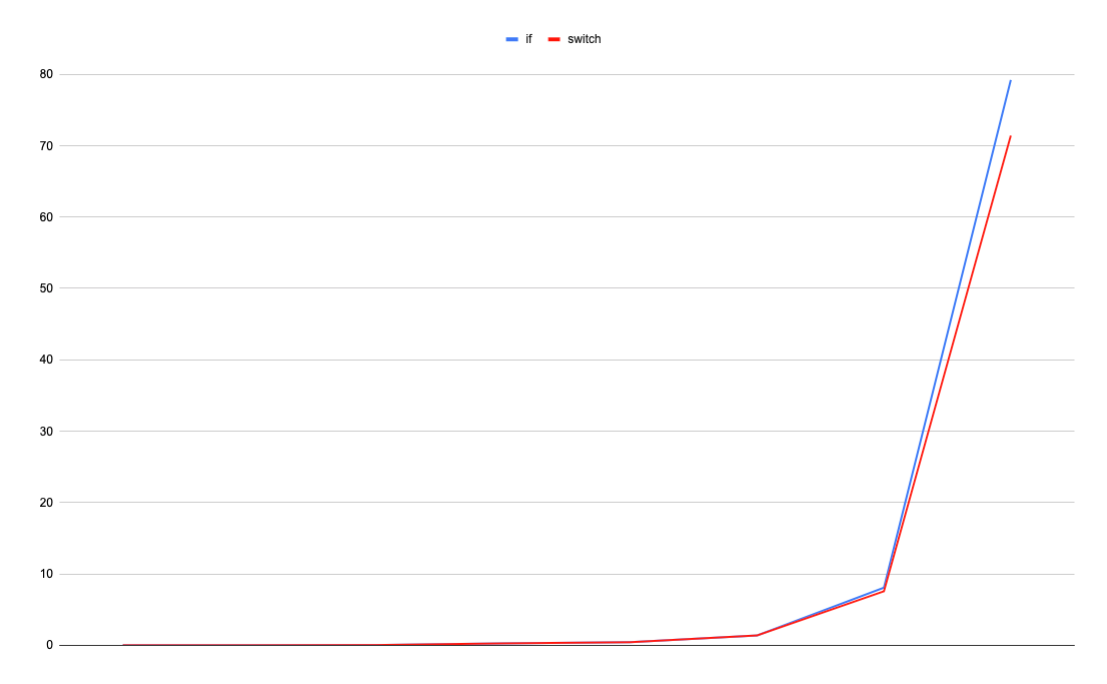
\includegraphics[width=\textwidth]{grafica_if_switch}
                \caption{Gráfica comparativa if-else vs switch}
            \end{figure}

            \begin{center}
                \begin{tabular}{ |c|c|c| }
                    \hline
                        iterations & if & switch \\
                        \hline\hline
                        1 & 0.000243 & 0.000270 \\
                        \hline
                        10 & 0.002797 & 0.002485 \\
                        \hline
                        100 & 0.027775 & 0.027261 \\
                        \hline
                        1000 & 0.260075 & 0.261464 \\
                        \hline
                        10000 & 0.431544 & 0.425668 \\
                        \hline
                        100000 & 1.368561 & 1.374575 \\
                        \hline
                        1000000 & 8.070825 & 7.560718 \\
                        \hline
                        10000000 & 79.199539 & 71.409653 \\
                    \hline
                \end{tabular}
            \end{center}

            Como se puede ver en la gráfica, la diferencia no es apreciable hasta las 1000000 iteraciones, pero después
            pasa a casi 8 segundos de diferencia en 10000000 iteraciones. Por esta razón se ha decidido que la función
            utilice la estructura \textit{switch-case}.\newline

            Finalmente, debido a la manera en la que realizan las comprobaciones de qué botones y sensores son
            utilizados, aunque un \textit{switch-case} es más rápido, esta estructura se reserva para la versión del
            programa que reproduce los sonidos leyendo del teclado. En el programa que controla los sensores se utiliza
            una estructura \textit{if-else}.

        % subsection if-else vs switch (end)

    % section Decisiones (end)

    \section{Arduino} % (fold)
    \label{sec:Arduino}

        Para la recepción de las señales del sensor de presión RP c18.3, se plantean dos opciones, se puede utilizar
        la propia Raspberry Pi en la que se ejecuta el programa que maneja los sonidos o una Arduino Nano. En el
        proyecto resultante se utiliza finalmente la Arduino debido a dos razones principales.\newline

        La primera razón es el precio y la escalabilidad, una Raspberry Pi cuesta 39,95\euro{} mientras que una
        Arduino Nano cuesta 10\euro{}. Una Arduino Nano cuenta con menos pines de E/S, pero añadir una placa es más
        barato y sencillo que añadir una placa de Raspberry Pi.\newline

        La segunda razón es la implementación del programa que se encarga de el sensor de presión. En Internet se
        pueden encontrar ejemplos y tutoriales refiriéndose a cómo implementar el sistema en una Arduino, pero no
        es tan fácil encontrar información para hacerlo desde una Raspberry Pi.\newline

        Por estas razones se elige realizar la recepción de las señales del sensor de presión desde la Arduino,
        haciendo el proceso más sencillo y más barato.

        \subsection{Conexión} % (fold)
        \label{sub:Conexion}

            Para realizar la conexión de los sensores se utilizan cables de protoboard conectados de la siguiente
            manera:

            \begin{figure}[ht]
                \centering
                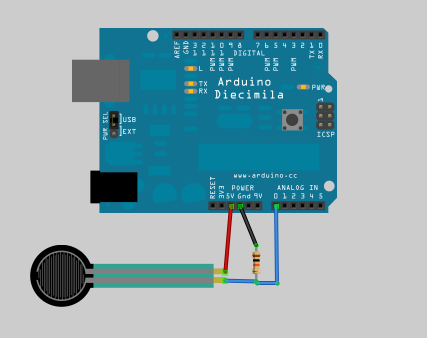
\includegraphics[width=\textwidth]{force_sensor_arduino}
                \caption{Esquema de conexión de sensores de presión\cite{force_sensor_arduino}}
            \end{figure}
        
        % subsection Conexión (end)

    % section Arduino (end)

% chapter Diseño (end)

%%%%%%%%%%%%%%%%%%%%%%%%%%%%%%%%%%%%%%%%%%%%%%%%%%%%%%%%%%%%%%%%%%%%%%%%%%%%%%%%%
% Implementación
%%%%%%%%%%%%%%%%%%%%%%%%%%%%%%%%%%%%%%%%%%%%%%%%%%%%%%%%%%%%%%%%%%%%%%%%%%%%%%%%%

\chapter{Implementación de la propuesta}
\label{cha:Implementacion}

    Poner especial atención al proceso: dificultades y problemas encontrados y cómo se han solucionado

        \section{Pads} % (fold)
        \label{sec:Pads}

            Los pads son las superficies que son golpeadas para generar los sonidos. Para este proyecto se han fabricado
            usando madera, cola y gomaeva\cite{GomaEva}. El coste total es de fabricar dos pads es de 3,09\euro{}.
            Comparado con otros productos similares como los de Prologix\cite{practice_pad}, cuyo kit de práctica de 4
            pads cuesta \$224,99, el precio de la solución propuesta en este proyecto es sensiblemente inferior.

        % section Pads (end)

        \section{Coste y presupuesto} % (fold)
        \label{sec:CosteYPresupuesto}

            tabla con el coste de desarrollo (incluye tu mano de obra... etc.)

        % section Coste y presupuesto (end)

        \section{Materiales} % (fold)
        \label{sec:Materiales}

            \begin{itemize}
                \item Dos hojas de goma eva: 1,20\euro{}
                \item Tres tablas madera MDF 600x300x10 mm: 7,47\euro{}
                \item Cables protoboard: 2,60\euro{}
                \item Sensor de fuerza Exing c18.3: 5,91\euro{}
                \item Tres sensores de fuerza Exing RP de S40: 50,95\euro{}
                \item Raspberry Pi 3B: 39,95\euro{}
                \item Tarjeta micro SD 8 GB: 5\euro{}
                \item Caja Aukru + cable alimentación: 11,99\euro{}
                \item Dos Arduino Nano: 30,86\euro{} (incluye gastos de envío)
            \end{itemize}

        % section Materiales (end)

        \section{Tiempo} % (fold)
        \label{sec:Tiempo}

            Para medir el tiempo que ha llevado realizar este trabajo, se ha utilizado la aplicación
            Clockify\cite{clockify}.\newline

            En total se han utilizado 74 horas y 24 minutos.%%%%%%%%%%%%%%%%%%%%%%%%%%%%%%%%%%%%%%%%%%%%%%%%%%%%%%
            %%%%%%%%%%%%%%%%%%%%%%%%%%%%%%%%%%%%%%%%%%%%%%%%%%%%%%%%%%%%%%%%%%%%%%%%%%%%%%%%%%%%%%%%%%%%%%%%%%%%%%
            %%%%%%%%%%%%%%%%%%%%%%%%%%%%%%%%%%%%%%%%%%%%%%%%%%%%%%%%%%%%%%%%%%%%%%%%%%%%%%%%%%%%%%%%%%%%%%%%%%%%%%

        % section Tiempo (end)

% chapter Implementación (end)

%%%%%%%%%%%%%%%%%%%%%%%%%%%%%%%%%%%%%%%%%%%%%%%%%%%%%%%%%%%%%%%%%%%%%%%%%%%%%%%%%
% Resultados y discusión
%%%%%%%%%%%%%%%%%%%%%%%%%%%%%%%%%%%%%%%%%%%%%%%%%%%%%%%%%%%%%%%%%%%%%%%%%%%%%%%%%

\chapter{Resultados y discusión}
\label{cha:ResultadosyDiscusion}

    -> Identifica los aspectos éticos y sociales relacionados con la profesión

% chapter Resultados y discusión (end)

%%%%%%%%%%%%%%%%%%%%%%%%%%%%%%%%%%%%%%%%%%%%%%%%%%%%%%%%%%%%%%%%%%%%%%%%%%%%%%%%%
% Conclusiones
%%%%%%%%%%%%%%%%%%%%%%%%%%%%%%%%%%%%%%%%%%%%%%%%%%%%%%%%%%%%%%%%%%%%%%%%%%%%%%%%%

\chapter{Conclusiones}
\label{cha:Conclusiones}

    Llegamos al final del proyecto. Durante los meses que se han invertido en la realización del trabajo, se han
    aprendido varias tecnologías y áreas.

    Se ha aprendido a conectar y programar sensores a placas Raspberry Pi y Arduino. Siguiendo con este tema, se ha
    visto cómo conectar los dos sistemas, para que la Arduino envíe información a la Raspberry Pi para el tratamiento de
    los datos recogidos por los sensores instalados en la Arduino.

    Por otro lado, se ha aprendido a reproducir archivos de sonido en entornos Linux/Unix de manera eficiente y
    simultánea utilizando el lenguaje de programación C.

    Finalmente, se ha alcanzado un resultado que cumple con los objetivos que se marcaron al comienzo del trabajo.
    Utilizando lo aprendido anteriormente, se logra una experiencia de tocar la batería parecida a la realidad,
    incluyendo la construcción de una batería física que poder tocar.

    \section{Trabajo futuro} % (fold)
    \label{sec:TrabajoFuturo}

        Durante la realización de este proyecto, ha surgido una serie de ideas que mejorarían la experiencia de tocar la
        batería, pero que, por falta de tiempo, no ha sido posible desarrollar. Las más destacables son:

        \begin{itemize}
            \item \textbf{Creación de una interfaz web:} Esta interfaz web podría utilizarse para arrancar y pausar la
            batería de forma sencilla, sin necesidad de entrar a la terminal para ello.
            \item \textbf{Sonidos personalizados:} Añadir un apartado a la interfaz web que permitiera al usuario
            añadir sus propios sonidos personalizados para configurar la batería a su gusto.
            \item \textbf{Aprender canciones:} Mediante una serie de LEDs, que se encienden en el momento preciso, se
            añadiría una canción a la batería y el usuario aprendería a tocarla de forma sencilla. Encendiendo el LED
            del pad que haya que tocar y apagándolo cuando haya sido tocado.
            \item \textbf{Guardar canción tocada:} Grabar lo que toque el usuario durante una cantidad limitada de
            tiempo en un archivo de audio para poder reproducirlo más tarde.
        \end{itemize}

    % section Trabajo futuro (end)

% chapter Conclusiones (end)

\newpage


\bibliographystyle{plain}
\bibliography{referencias}

\end{document}
